\section{Methods Supplemental Information}

\subsection{Microwave Scattering (MWS) Setup}

\begin{figure}[]
\centering
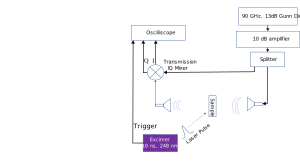
\includegraphics[width=0.8\textwidth]{\repodir/final/figures/SI/output/MWS_Setup.png}
\caption{Microwave scattering setup.}
\label{fig:SI_MWS_Setup}
\end{figure}

The microwave scattering setup is shown in \ref{fig:SI_MWS_Setup_Silicon}. The parts were ordered from Erevant, formerly Sage Millimeter. The system is W-band and based on WR-10 waveguides. The microwave source is a 90 GHz Gunn oscillator (SOM-90305213-10-S1) with an output power of +13 dBm. The output of this source is fed into a 10 dB gain, +15 dBm P1dB, in-line waveguide power amplifier (SBP-7531141015-1010-E1). The output of the power amplifier is then fed into a 4-way in-line power divider (SWP-90310404-10-E1). In the current configuration, only two outputs of the power divider are used, and the remaining two are terminated with waveguide terminators (TODO). One power of the power divider is used for the main transmitted power, which is sent through waveguides to a horn (TODO) that transmits the microwaves into free space. The transmitted microwaves after the sample are collected by the same type of horn, and the collected microwaves are sent to the IQ mixer (SFQ-75311415-1010SF-N1-M). The LO input of the IQ mixer is fed by the remaining port of the power divider. Between the power divider and the LO input there is a phase shifter (STP-18-10-M2) that is typically used to maximize the I signal in the absence of a sample. 

The I and Q signals from the oscilloscope are fed directly into a Teledyne Leroy WavePro 404HD-MS Oscilloscope. The oscilloscope utilized 1 MOhm impedance. (TODO) The oscilloscope is triggered from the excimer laser. 

% https://netldoe.sharepoint.com/sites/MHDLab/_layouts/OneNote.aspx?id=%2Fsites%2FMHDLab%2FSiteAssets%2FMHD%20Lab%20Notebook&wd=target%28HVOF%20Booth.one%7C926BAC12-30AE-4CC1-87A1-28B752C7F9AD%2FMeasurements%7C427606CE-8CD2-43D7-A8DB-6C8D894FFC45%2F%29onenote:https://netldoe.sharepoint.com/sites/MHDLab/SiteAssets/MHD%20Lab%20Notebook/HVOF%20Booth.one#Measurements&section-id={926BAC12-30AE-4CC1-87A1-28B752C7F9AD}&page-id={427606CE-8CD2-43D7-A8DB-6C8D894FFC45}&end

The excimer laser is sent through a 90/10 UV beam splitter with the 10 \% sent to a photovoltaic power meter (Ophir PD-10C), however the power data was not used in this analysis. The remaining 90 \% of the laser is directed through a Thorlabs FW 102C Filter Wheel. The filter wheel housed Thorlabs reflective UV neutral density filters. These neutral density filters have been observed to degrade from continued use with the excimer laser, and the laser power was measured before an after the experiment to ensure there was no significant degradation in filter performance. After the filter wheel, the laser is redirected with a UV mirror (Acton Instruments, TODO) to the center of the microwave horns. Everything including the final mirror is located on the motorized stage, which moves parallel to the torch axis.  

The distance between the horns is 85.725 mm. The mirror that sends the excimer beam to the measurement location is located 247 mm downstream along the torch axis, 397 mm horizontally (along the table) perpendicular from the torch axis, and 65 mm vertically above the torch axis. 

On each date, the microwave transmission magnitude with nothing in between the horns, $U_{nothing}$, was measured. During these measurements all other settings the same (excimer laser, oscilloscope, etc.) compared to the main experimental measurements, except that the oscilloscope time window may be 250 $\mu s$ used for the Silicon measurements may have been used. An example measurement of $U_{nothing}$ is shown in \ref{fig:SI_MWS_nothing_time_trace}. For approximately 1 $\mu s$ there is electronic interference from the laser pulsing, which also appears in the main experimental transmission measurements. 



\begin{figure}[]
\centering
\includegraphics[width=0.8\textwidth]{\repodir/final/dataset/output/figures/mws_nothing_time_trace_2023-05-18.png}
\caption{Time trace from 2023-05-18 of the transmission measurement without any free jet.}
\label{fig:SI_MWS_nothing_time_trace}
\end{figure}

On 2023-05-24 the transmission was measured as a function of position as shown in \ref{fig:SI_MWS_nothing_motor}. There is a slight increase in transmission when the stage is moved as close as possible to the barrel exit, possibly due to reflections from the barrel.


\begin{figure}
\centering
\includegraphics[width=0.8\textwidth]{\repodir/final/dataset/output/figures/mws_nothing_motor_2023-05-24.png}
\caption{Motorized stage for position dependent transmission measurements.}
\label{fig:SI_MWS_nothing_motor}
\end{figure}


The  measured at the nominal position (180 mm) for each of the dates is presented in \ref{fig:SI_MWS_nothing_T0}A. Note that for 2023-05-12, the measurement was only taken at the barrel exit, which is corrected by a factor of 0.95 to estimate the transmission at the nominal position. This factor is determined from the ratio of the transmission at the nominal position to the transmission at the barrel exit from figure \ref{fig:SI_MWS_nothing_motor}.

\ref{fig:SI_MWS_nothing_T0}B shows the absolute transmission of the magnitude before the laser pulse for the case 536\_pos, for different dates. The transmission is then measured with the sample in place. The transmission is then calculated as the ratio of the sample transmission to the transmission with nothing in place. An example of this is shown in \ref{fig:SI_MWS_nothing_T0}.  




\begin{figure}[]
\centering
\includegraphics[width=0.8\textwidth]{\repodir/final/analysis/output/figures/mws_nothing_T0.png}
\caption{A) Measurement of transmission without any torch, B) position dependent transmission measurement.}
\label{fig:SI_MWS_nothing_T0}
\end{figure}


\ref{fig:SI_mws_processing_overview} shows the processing steps for the MWS data. 

\begin{figure}[]
\centering
\includegraphics[width=0.8\textwidth]{\repodir/experiment/analysis/mws/output/figures/mws_processing_overview.png}
\caption{Microwave processing overview}
\label{fig:SI_mws_processing_overview}
\end{figure}


Before each experiment we performed measurements with a silicon sample in the location of the torch to ensure the system was functioning properly. The silicon measurements are shown in \ref{fig:SI_MWS_Silicon}. 

\begin{figure}[]
\centering
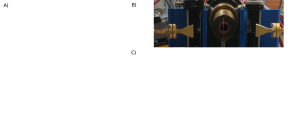
\includegraphics[width=0.8\textwidth]{\repodir/final/figures/SI/output/MWS_Silicon.png}
\caption{Silicon Measurements}
\label{fig:SI_MWS_Silicon}
\end{figure}




\begin{figure}
\centering
\includegraphics[width=0.8\textwidth]{\repodir/experiment/analysis/mws/resampling/output/figures/mws_sample_nors_compare.png}
\caption{Comparison of the resampling methods.}
\label{fig:SI_mws_resampling}
\end{figure}


\begin{figure}
\centering
\includegraphics[width=0.8\textwidth]{\repodir/experiment/analysis/mws/output/figures/mws_fitting_compare.png}
\caption{Comparison of the fitting methods for the monomolecular regime. Fit to an exponential model and full solution of differential equation. }
\label{fig:SI_mws_fitting_compare}
\end{figure}

\clearpage
\subsection{Laser Profile}


\begin{figure}[H]
\centering
\includegraphics[width=0.8\textwidth]{\repodir/experiment/analysis/mws/output/figures/laser_profile.png}
\caption{Laser profile measurement}
\label{fig:SI_Laser_Profile}
\end{figure}

\clearpage
\subsection{Absorption Emission Spectroscopy (AES) Setup}




Ocean Optics HR4000 Spectrometer. 

Ocean Optics MPM-2000-UV-VIS600-2X8 Multiplexer. The LED output and spectrometer input are both connected to the multiplexer for both AES diagnostics (barrel exit and MWS measurement location). The multiplexer continuously switches between the locations every 10 seconds throughout the duration of the measurement. 


The LED is a Thorlabs M780F2 780 nm LED. The LED is driven by a Thorlabs T-Cube LED Driver. The LED is triggered by the spectrometer. The LED is continuously turned on and off throughout the experiment to obtain LED on and LED off measurements. The when switching the LED, there is a 1 second delay before the spectrometer is triggered to allow the LED state to stabilize. This LED switching time limits the temporal resolution of the AES measurements and fluctuations in the free jet seed level between the LED on and off measurements can cause unphysical results, such as negative absorption. 




Figure \ref{fig:SI_AES_proc_overview} shows the processing steps for the AES data.

\begin{figure}[]
    \centering
    \includegraphics[width=0.8\textwidth]{\repodir/experiment/analysis/absem/output/figures/absem_proc_overview.png}
    \caption{AES processing overview}
    \label{fig:SI_AES_proc_overview}
\end{figure}


\subsection{Photodiode (PD) Setup}

Figure \ref{fig:PD_setup_schematic} shows the photodiode setup schematic. All parts were ordered from Thorlabs. The light is collected and then collimated into the beam splitter with F110SMA-780 fiber coupled lens with 780 nm f = 6.24 mm and NA = 0.37 SMA. The fiber coupled lenses are connected to a Thorlabs 600 um 0.39 NA optical fiber. The light is split with a CCM1-BS014 beam splitter into two separate photodiode pathways that are intended to collect the potassium emission peak as well as the emission off-peak for comparison. Each pathway consists of a bandpass filter and placed before a SM05PD1A Cathode Grounded Silicon Photodiode. (TODO: fixed size iris? ). AThe photodiodes are powered with a PBM42 bias module powered by ? V (TODO). The photodiode signals are amplified with AMP101 Transimpedance amplifiers set to an amplification of 100 kV/A. This signal is then sent to channels 3 and 4 of the oscilloscope, where channels 1 and 2 are used for the MWS  I and Q measurements.



\begin{figure}[]
    \centering
    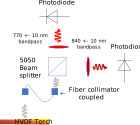
\includegraphics[width=0.8\textwidth]{\repodir/final/figures/schematics/output/PD_setup.png}
    \caption{Photodiode (PD) setup schematic.}
    \label{fig:SI_PD_setup_schematic}
\end{figure}



\begin{figure}[]
    \centering
    \includegraphics[width=0.8\textwidth]{\repodir/final/figures/setup_images/Photodiode_Setup.png}
    \caption{Image of the photodiode setup}
    \label{fig:SI_PD_setup_image}
\end{figure}






\clearpage
\subsection{Emulsion Preparation and Delivery}

Potassium was introduced into the HVOF system by creating a potassium carbonate (K2CO3) brine and kerosene emulsion. This emulsion was delivered into the HVOF fuel flow via a tee. The tee run carried the fuel flow while the tee branch accepted emulsion through a PTFE feed line which was served by a high-pressure syringe pump. Three syringes were manifolded together. A switching valve allowed syringes to withdraw emulsion from the stirred reservoir or to infuse emulsion into the HVOF fuel line. Before, igniting the torch, the ?m emulsion line was filled. At the tee, fuel flow momentum was used to mix the emulsion with the fuel flow over the ?cm distance between the tee and combustion chamber nozzle. 


distributing brine droplets within part of the fuel supply via a water-in-oil emulsion (W/O). A droplet of W/O emulsion might be expected to pass through the combustor atomizer and promptly evaporate/burn from outer surface in. High surface to volume ratio, as well as close contact with the fuel should help the brine promptly evaporate, freeing the K2CO3 to dissociate, releasing gaseous, metallic potassium. To the extent the water boils after kerosene, water flashing to steam can break up kerosene droplets in the combustor and increase the effectiveness of mixing there. 

Literature was reviewed for an emulsion specifically designed to work with brine – especially water-in-oil (W/O) emulsions.  Developing emulsions for use in oilfields, Mohamed et al.\cite{mohamedInfluenceSurfactantStructure2017a} investigated high salinity W/O emulsions between “formation brine” and diesel. According to these authors, “[D]iesel and kerosene are used in the oilfields because of availability.” Their formation brine included more than 221,673 mg total dissolved solids (TDS) per liter of brine (~20% by mass).  

We noted the most stable result in ​[1]​ “reproduced” it using a potassium carbonate brine, kerosene, and a SPAN 80 / TWEEN 80 surfactant blend meeting their recommended HLB of 6.8. The concentration of the surfactant was 0.5% of the emulsion by volume - the minimum necessary found in [1] to obtain a stable emulsion. (Mohamed et al. measured ~5% of liquid came out of emulsion in 100 minutes at 120 °C).  

To generate the initial brine droplets, we used a spray nozzle. Spraying to create an emulsion is an age-old practice \cite{atkinsonKeroseneEmulsionHow1890} with relevance here because it avoids the temperature-rise associated with higher energy processes. These spray-generated droplets were then passed through an ultrasonic process to break them up further. This continuous process also minimized temperature rise because the material exited seconds after entering the ultrasonic field. 

The emulsion preparation process is given below:

Makes 500 mL 

1 . Prepare liquid components ahead of time 
\begin{itemize}
\item 100g supply of surfactant blend with HLB=6.8 by mixing 77g of Span 80 and 23g of Tween 80 on a magnetic stir plate 

\item Eight aliquots of K2CO3 brine by mixing 847.7g of K2CO3 powder into 350mL of deionized water on a magnetic stirrer 

\item Eight aliquots of prepared kerosene by mixing 5g of the surfactant blend into 106.5g of kerosene  

\item Each Brine/Kerosene aliquot pair will produce 500mL of emulsion. 
\end{itemize}


2. Prepare a 2-liter supply for a seeded firing experiment 

\begin{itemize}
    
\item Decant an aliquot of prepared kerosene into a beaker and begin stirring on a magnetic stir plate. 

\item Pump (peristaltic)the aliquot of K2CO3 brine through a spray nozzle, producing a mist of droplets to fall into the prepared kerosene. Droplet/kerosene interfaces adsorb the surfactant to make a relatively fine pre-emulsion. 

\item While continuing to magnetically stir, pump the pre-emulsion through an ultrasonic continuous flow cell to further break up the dispersed brine droplets. 

\item Batches were generally stored overnight and combined in magnetically stirred reservoir at the beginning of the photoionization experiment. 
\end{itemize}


The following emulsion recipe was used. The mass density (rho) was measured by withdrawing ? ml of emulsion and weighing it. 

The mass of the fuel was incorrectly used as 109 g to calculate setpoints on on each day except 2023-05-24, instead of 106.5 g. TODO: Was this actually used in the emulsion?



\begin{table}[h]
\centering
\begin{tabular}{|l|l|l|}
\hline
\textbf{Parameter} & \textbf{2023-04-07 to 2023-05-18} & \textbf{2023-05-24} \\
\hline
M\_K2CO3 & 84.7 gram & 84.7 gram \\
M\_fuel & 109.0 gram & 106.5 gram \\
M\_water & 350.0 gram & 350.0 gram \\
M\_span80 & 3.84 gram & 3.84 gram \\
M\_tween80 & 1.17 gram & 1.17 gram \\
rho & 1.056 gram / milliliter & 1.056 gram / milliliter \\
M\_surf & 5.01 gram & 5.01 gram \\
M\_brine & 434.7 gram & 434.7 gram \\
M\_total & 548.71 gram & 546.21 gram \\
f\_fuel & 0.19864773742049532 dimensionless & 0.19497995276541988 dimensionless \\
f\_K2CO3 & 0.15436204916987115 dimensionless & 0.15506856337306163 dimensionless \\
\hline
\end{tabular}
\caption{Emulsion Parameters}
\label{tab:emulsion_parameters}
\end{table}

\subsection{Additional Experiment Pictures}

\begin{figure}[]
\centering
\includegraphics[width=0.8\textwidth]{\repodir/final/figures/setup_images/2023-05-18_Full_Setup_Topcam_2.png}
\caption{Full setup with top camera. Taken on 2023-05-18.}
\label{fig:SI_Full_Setup_Topcam}
\end{figure}

\begin{figure}[]
\centering
\includegraphics[width=0.8\textwidth]{\repodir/final/figures/setup_images/2023-05-24_PI_Setup.png}
\caption{Full view of experiment setup. Taken on 2023-05-24.}
\label{fig:SI_Full_Setup_PI}
\end{figure}

% final/figures/setup_images/2023-05-24_Rear_View.png

\begin{figure}[]
\centering
\includegraphics[width=0.8\textwidth]{\repodir/final/figures/setup_images/2023-05-24_Rear_View.png}
\caption{Rear view of experiment setup. Taken on 2023-05-24. The optical processing setup (beam splitter, filters, and photodiode) of the PD diagnostic can be seen on the table. }
\label{fig:SI_Rear_View}
\end{figure}

\begin{figure}[]
\centering
\includegraphics[width=0.8\textwidth]{\repodir/final/figures/setup_images/2023-05-18_Top_View.jpg}
\caption{Top view of experiment setup. Taken on 2023-05-18.}
\label{fig:SI_Top_View}
\end{figure}


